\chapter{A Critique of the Master Sintering Curve Analysis of Sintering Processes}

\section{Introduction}
The master sintering curve (MSC) approach was developed by Su and Johnson \cite{Su1996} to generalize densification behavior of a sintering powder with a single curve for the entire sintering time/temperature profile. The MSC approach is based on a combined-stage sintering model developed by Hansen et al, \cite{Hansen1992} given as:

%%
\begin{equation}
\label{Ch6-eq: eq1}
\frac{1}{\rho} \frac{d\rho}{dt} = \frac{3 \gamma \Omega}{k_{B}T} \left( \frac{\delta D_{b} \Gamma_{b}}{G^{4}} + \frac{D_{v} \Gamma_{v}}{G^{3}} \right)
\end{equation}
%%

\noindent where $\rho$ is relative density of the powder compact, $d\rho/dt$ is densification rate, $\gamma$ is surface energy, $\Omega$ is molar volume, $k_{B}$ is Boltzmann's constant, $T$ is absolute temperature, $G$ is grain size, $D$ is diffusion coefficient, $\delta$ is grain boundary thickness, and $\Gamma$ is a geometric scaling factor. The subscripts $b$ and $v$ represent grain boundary and volume diffusion mechanisms, respectively. The MSC was originally derived to simplify the combined-stage sintering model (Eq. \ref{Ch6-eq: eq1}) to account for only a single diffusion mechanism, and by considering diffusion as thermally-activated with an activation energy $Q$. The resulting equation is given as:

%%
\begin{equation}
\label{Ch6-eq: eq2}
\frac{1}{\rho} \frac{d\rho}{dt} = \frac{3 \gamma \Omega}{k_{B}T} \left( \frac{D \Gamma}{G^{n}} \right)
\end{equation}
%%

\noindent where

%%
\begin{equation}
\label{Ch6-eq: eq3}
D = D_{0}e^{-Q/RT}
\end{equation}
%%

\noindent and $R$ is the ideal gas constant. Eq. \ref{Ch6-eq: eq2} is re-written to collect microstructural parameters on the left hand side and temperature dependent parameters on the right hand side:

%%
\begin{equation}
\label{Ch6-eq: eq4}
\frac{k_{B} G^{n}}{3 \rho \gamma \Omega \Gamma D_{0}} \frac{d\rho}{dt} = \frac{1}{T} exp \left( -\frac{Q}{RT} \right) = \frac{d \Theta}{dt}
\end{equation}
%%

\noindent Eq. 4 can be integrated to give:

%%
\begin{equation}
\label{Ch6-eq: eq5}
\frac{k_{B} }{ \gamma \Omega \Gamma D_{0}} \int_{\rho_{0}}^{\rho} \frac{(G(\rho))^{n}}{3 \rho \Gamma (\rho)} d \rho = \int_{0}^{t} \frac{1}{T} exp \left( -\frac{Q}{RT} \right) dt = \Theta
\end{equation}
%%

\noindent Equation \ref{Ch6-eq: eq5} describes the sintering behavior for an arbitrary time-temperature profile, and the integral over this profile with respect to time is termed the work of sintering $\Theta$. The MSC is obtained by plotting $\rho$ versus $\Theta$. The left hand side of Eq. \ref{Ch6-eq: eq4} is not solved, because many of the parameters are unknown. However, as long as these parameters are independent of time and temperature, data plotted in this way will collapse into a single continuous curve for a single value of $Q$. It is interesting to note that the MSC analysis is independent of the sintering mechanism and, as a generalized model, was applied to other thermally activated process such as grain growth \cite{Park2006} and binder decomposition \cite{Diantonio2005,Aggarwal2007}.

In practice, $Q$ is a fitting parameter for which the best-fit MSC is obtained over a range of heating rates by determining the minimum mean residual. Assuming arbitrary values for $Q$ in Eq. \ref{Ch6-eq: eq5}, the mean residual square is calculated by \cite{Blaine2006}

%%
\begin{equation}
\label{Ch6-eq: eq6}
\mbox{Mean residual square} = \sqrt{\frac{1}{\rho_{s}-\rho_{0}}\int_{\rho_{0}}^{\rho_{s}} \frac{\Sigma_{i=1}^{N} \left( \frac{\Theta_{i}}{\Theta_{avg}}-1 \right)^{2}}{N} d\rho}
\end{equation}
%%

\noindent where $N$ is the number of experimental data points gathered at a series of heating rates and a sintered density $\rho_{s}$, and $Q_{avg}$ is the average of all $Q_{i}$ over $N$. The $Q$ value that yields the minimum mean residual square is the $Q$ value at which the MSC trajectories obtained from the densification curves at different heating rates yield the best fit and converge onto a single curve.  Because of the mechanistic nature of the model, the $Q$ parameter is usually referred to in the literature as the 'activation energy' for sintering.

MSC analysis has been applied to ceramic powders formed and densified by a variety of techniques. For high purity alumina, the reported $Q$ values vary drastically, as seen in Table \ref{Ch6-table:table1}. In Su and Johnson’s original work \cite{Su1996a}, $Q$ values of 440 and 488 kJ/mol were determined by minimum mean residuals and isostrain analysis, respectively, for an ultrafine, ultrahigh purity alumina (AKP-50, Sumitomo Chemical America, Inc.), showing that the activation energy obtained from minimum mean residuals is in close agreement with the activation energies determined by conventionally used methods. Using the same powder, Tatami et al. \cite{Tatami2006} determined a $Q$ of 555 kJ/mol, and when the powder was doped with 2000 ppm MgO, a $Q$ of 880 kJ/mol was determined. Pouchly et al. \cite{Pouchly2009} estimated the $Q$ of two different ultrahigh purity alumina powder graded (Taimicron TM-DAR, Taimei Chemicals and RC-HP DBM, Reynolds Chemicals) to be 770 and 640 kJ/mol, respectively, and attributed the difference in $Q$ to the difference in particle size of 110 nm and 240 nm, respectively. Aminzare et al. \cite{Aminzare2010}, reported $Q$ values of 700 and 605 kJ/mol for alumina (Taimicron TM-DAR, Taimai Chemicals) samples prepared by dry pressing and pressure filtration, respectively. Using the same alumina powder grade (Taimicron TM-DAR, Taimai Chemicals), Guillon and Langer \cite{Guillon2010} reported a $Q$ of 290 kJ/mol for Al$_{2}$O$_{3}$ densified by spark plasma sintering (SPS). They attributed the lower $Q$ value to the effect of the high heating rates of 35 – 150 $^{\circ}$C/min during SPS. $Q$ values of up to 1064 kJ/mol were reported by Shao et al. \cite{Shao2009} for granulated and dry pressed alumina powder (350 nm, 99.9\%, Dalian Luming Nanometer Material Ltd.). They explained the higher $Q$ values as an effect of slower heating rates (0.5 and 5 $^{\circ}$C/min) on densification.

The effect of heating rate on densification was explained by Harmer and Brook \cite{Harmer1981} as due to the relative time the material is heated under conditions favoring surface and grain boundary diffusion. They reasoned that a slow heating process favors surface diffusion and particle coarsening because surface diffusion usually has a lower activation energy than densifying mechanisms like grain and volume diffusion. Samples heated at slow rates spend relatively longer times at lower temperatures and, therefore, experience more particle coarsening prior to reaching the temperatures where densification occurs. Thus, the sintering driving force from surface area is higher during the densification stage when ceramics are fired at higher heating rates since these samples do not undergo as much coarsening prior to densification. In MSC analysis, these relative changes in mechanism result in lower $Q$ values at faster heating rates. However, it is assumed in the MSC analysis that sintering occurs by a single mechanism for the heating conditions used to collect densification data. Since data for MSC analysis is performed by heating samples at different heating rates, the contributions from surface diffusion and grain boundary diffusion vary, and it is questionable if the $Q$ values obtained can be used for mechanistic interpretations. Furthermore, it is not apparent why there is so much variability of the reported $Q$ values.  

In this chapter, we investigate how forming techniques and powder chemistry affect the $Q$ parameter and the shape of the MSC for a commercial specialty alumina powder. We explore how forming process-induced differences in relative green density, microstructural homogeneity and shrinkage anisotropy affect the value of $Q$. We also investigate how the assumption of a constant microstructure (i.e., grain size) at high density affects the MSC fit and $Q$ value. A series of Na$_{2}$O-doped samples were studied to determine how changes in densification mechanism affect the value of $Q$.  Based on these experiments, we discuss the limits and accuracy of the MSC approach and then determine how MSC can be used in a constructive, practical way to predict the sintering of a specific powder.

\section{Experimental Procedure}

To examine the impact of the forming technique on the MSC, we prepared undoped alumina (CT3000LS-SG, Almatis, Inc., Leetsdale, PA) samples by dry pressing, slip casting and tape casting. The powder was a Bayer process alumina (99.8\%) with an average particle diameter of 0.3 $\mu$m. Two sets of samples were prepared by uniaxial dry pressing. For one set, the as-received powder was sieved to -106 $\mu$m and uniaxially dry pressed at 30 MPa. The powder handling for the second set was designed to produce a soft, granuled powder by dispersing it in ethanol with 5 wt.\% polyethylene glycol (PEG 600 (?), Alfa Aesar, Ward Hill, MA, USA). After ball milling for 24 h, the dried powder was sieved to -106 $\mu$m and samples were lightly pressed at 30 MPa.  Both sample types were isopressed at 200 MPa after removing the organic processing aids by heating at 600$^{\circ}$C for 12 h in air.

For tape casting, a slurry was prepared by ball milling 68.14 wt.\% alumina powder with 15.31 wt.\% xylene (ACS Reagent grade, Avantor Performance Materials, Inc., Center Valley, PA, USA), 15.31 wt.\% ethanol (200 proof), and 1.24 wt.\% blown menhaden fish oil (Grade Z-3, Tape Casting Warehouse, Morrisville, PA, USA). After 24 h, 3.09 wt.\% polyvinyl butyral (PVB B-98, Tape Casting Warehouse, Morrisville, PA, USA), 1.55 wt.\% polyalkylene glycol (PAG, UCON50HB2000, Tape Casting Warehouse, Morrisville, PA, USA) and 1.55 wt.\% butyl benzyl phthalate (BBP S-160, Tape Casting Warehouse, Morrisville, PA, USA) were added and the mixture was ball milled for another 24 h, before 1 drop of cyclohexane (99+\%, Alfa Aesar, Ward Hill, MA, USA) per 20 g of alumina powder was added and the slurry was stirred for an additional 45 min. The slurry was tape cast on a silicone-coated Mylar$^{TM}$ carrier tape using a doctor blade gap height of 305 $\mu$m. After drying, the tape was cut, stacked, uniaxially pressed at 70$^{\circ}$C for 10 min at minimal pressure to tack the layers together, and then isostatically laminated at 74$^{\circ}$C and 20 MPa for 30 min.

For non-aqueous slip casting, 65.3 wt.\% powder was dispersed in Xylene with 2 wt.\% Menhaden fish oil, ball milled for 24 h, and slip cast. For aqueous slip casting 76 wt.\% alumina powder was dispersed in deionized water with 3 wt.\% Darvan C (R. T. Vanderbilt Company, Inc., Norwalk, CT, USA). The pH of the Darvan and water mixture was adjusted to 11 using 5 M NH$_{4}$OH before the alumina powder was added. The slurry was ball milled for 24 h and then slip cast. In both cases the mold consisted of a PVC tube (20 mm diameter) on a plaster of Paris plate.

The polymer processing aids were burned out of all samples by heating at 600$^{\circ}$C for 12 h in air. All samples were cold isostatically pressed at 200 MPa (CIP, Autoclave Engineers, Erie, PA). The samples were subsequently cut and ground into 3 x 3 x 15 mm3 bars for dilatometry studies. The long axis of the dilatometry samples corresponds to the pressing direction during uniaxial compaction, the casting direction during slip casting, and the casting direction for tape cast samples. The bars were heated to 1525$^{\circ}$C or 1600$^{\circ}$C at 5, 10, and 20$^{\circ}$C/min in a thermomechanical analyzer (TMA; Linseis PT1600, Robbinsville, NJ) to record the linear shrinkage of the samples. The thermal expansion contribution of the samples to the dilatometry curves was subtracted from the dimensions measured in-situ using the cooling curves of the samples measured in the TMA.

To examine how changes in chemistry affect the MSC analysis, we studied a series of dry pressed Na$_{2}$O-doped aluminas. The alumina powder was doped with up to 1000 ppm Na$_{2}$O using sodium acetate (NaC$_{2}$H$_{3}$O$_{2}$*3H$_{2}$O, ACS grade, BDH, West Chester, PA). The detailed doping procedure is reported in chapter 2.


\section{Results and Discussion}

\subsection{The effect of forming on $Q$}
During initial studies, we observed different degrees of anisotropic shrinkage as a function of the forming method. For example, the dilatometry curves of the non-aqueous slip cast samples during heating to 1525$^{\circ}$C at 5, 10, and 20$^{\circ}$C/min are shown in Figure \ref{Ch6-figure:Figure1}. The shrinkage was measured in the z-direction, i.e., the direction parallel to the capillary (i.e. shear) force of the plaster of Paris mold during slip casting, and in the x/y-direction, perpendicular to the capillary force. Anisotropic shrinkage was observed for all heating rates. Samples heated at 5$^{\circ}$C/min have a higher shrinkage in the z-direction than in the x/y-direction throughout the entire sintering process, whereas samples heated at 10 and 20$^{\circ}$C/min show slightly more shrinkage in the x/y-direction in the initial stage of densification followed by a crossover in the shrinkage and much more shrinkage in the z-direction at higher densities. The anisotropic shrinkage was quantified with a shrinkage anisotropy factor $k$, which is the ratio of the shrinkage in the z-direction to the shrinkage in x/y-direction. Figure \ref{Ch6-figure:Figure2} shows how $k$ changes as a function of relative density and heating rate for the non-aqueous slip cast samples heated at different heating rates during densification. Interestingly, the shrinkage anisotropy factor changes significantly as a function of heating rate during densification and there is much less change in $k$ at the slowest heating rate. Relative density was calculated using the shrinkage anisotropy factor and is plotted as a function of temperature in Figure \ref{Ch6-figure:Figure3}. The mean residuals were calculated as a function of $Q$ (Eq. \ref{Ch6-eq: eq6}), and the minimum is at $Q$ = 550 kJ/mol (Figure \ref{Ch4-figure:Figure4}). The relatively sharp minimum provides evidence that a single MSC curve is a good fit for the measured TMA data. 

When shrinkage in the z-direction is assumed to represent isotropic shrinkage (i.e. $k$=1), then $Q$ increases to 625 kJ/mol. Figure \ref{Ch6-figure:Figure5} compares the MSCs obtained when the shrinkage anisotropy was accounted for (550 kJ/mol) or by assuming isotropic shrinkage (no correction for anisotropy). This example demonstrates the importance of determining whether the sample shrinks anisotropically during the density measurements used to construct the MSC, and the need to correct for anisotropic shrinkage to determine an accurate value $Q$ and MSC. Note that the curves at all 3 heating rates coincide.

Figure \ref{Ch6-figure:Figure6} shows the corresponding MSC curves of samples formed by various techniques and heated to 1525$^{\circ}$C. The measurements were corrected for shrinkage anisotropy as described above. The total shrinkage anisotropy was $\sim$0.75 for slip cast and tape cast samples, and $\sim$0.92 for dry pressed samples. It is clear that $Q$ changes as a function of forming technique, which is, in part, due to different green densities. The sample prepared by non-aqueous slip casting has a green density of 59\% and the lowest $Q$ (550 kJ/mol), followed by the sample prepared by aqueous slip casting with a green density of 58\% and a $Q$ of 650 kJ/mol. The samples prepared by dry pressing (no PEG) and tape casting have green densities of 57\% and 55\%, respectively, and both samples have a $Q$ of 730 kJ/mol. The dry pressed sample with 5 wt.\% PEG has a green density of 55\% and the highest activation energy with 810 kJ/mol. It can thus be observed that $Q$ decreases as the green density increases and that the shape and position of the MSC changes as a function of forming technique (Figure \ref{Ch6-figure:Figure6}). Aminzare et al. \cite{Aminzare2010} also observed that $Q$ is sensitive to the forming technique and concluded that samples prepared by pressure filtration have a lower $Q$ than dry pressed samples as a result of better sample homogeneity as evidenced by the higher green density. As shown in this work, the effect of green density on $Q$ is complicated. For example, the samples prepared by tape casting and dry pressing with 5 wt.\% PEG have the same green density of 55\%, but different $Q$ values of 730 kJ/mol and 810 kJ/mol, respectively, and different MSC shapes. This suggests that other sample characteristics, in addition to green density, influence $Q$, such as pore size, pore size distribution, and particle/pore orientation. 

\subsection{MSC at high densities}
The final densities used in the MSC analysis of the samples discussed above are $\leq$90\%. Above 90\% density we observed that the MSC curves for different heating rates diverge and thus which dramatically influences the value of $Q$. Figure \ref{Ch6-figure:Figure7}a shows the densification curves of dry pressed samples sintered to >95\% density when heated to 1600$^{\circ}$C at different heating rates. The minimum mean residual analysis yielded $Q$ = 700 kJ/mol (Figure \ref{Ch6-figure:Figure7}b) and Figure \ref{Ch6-figure:Figure7}c shows the resulting MSC. It can be seen that $Q$ = 700 kJ/mol gives a good fit at low densities, but the trajectories begin to diverge at densities >90\% (see Fig \ref{Ch6-figure:Figure7}c insert). 

To account for the effect of bulk density on densification we determined the activation energy at some relative densities by plotting $ln(-T·d\rho/dt)$ vs. $1/T$ and determining the slopes of the resulting linear curves of the isodensities. Figure \ref{Ch6-figure:Figure8} shows the development of the apparent activation energy obtained from iso-density analysis, $Q_{iso}$, and it can be seen that $Q_{iso}$ is $\sim$700 kJ/mol and increases slightly with increasing relative density. At densities >85\% $Q_{iso}$ increases somewhat more rapidly, and at densities >95\% $Q_{iso}$ increases drastically to >1800 kJ/mol. This change in $Q_{iso}$ explains the divergence of the MSC trajectories obtained from the different heating rates using $Q_{MSC}$ = 700 kJ/mol. 

At densities <90\% the activation energy obtained from the minimum mean residuals $Q_{MSC}$, which is used to obtain the MSC, is reasonably close to the activation energies obtained from the iso-density analysis, $Q_{iso}$, resulting in a good fit at all heating rates. However, at densities >90\% where we observe divergence in the MSCs, the values of $Q_{iso}$ are >100 kJ/mol greater than the $Q_{MSC}$ value used to construct the MSC. Although the idea of variable activation energy is understandable, it is not physically realistic to consider that the activation energy for sintering is intrinsically a function of $\rho$. It is more likely that this increase in $Q_{iso}$ and the divergence of the MSC at high densities is caused by microstructural or mechanistic changes that are not accounted for in the MSC model. 

\subsection{Quantification of the MSC shape}
A way to account for microstructural changes is analyzing the shape of the MSC, since it is determined by the evolution of the microstructural parameters in the left hand side of Eq. \ref{Ch6-eq: eq5}. Microstructural evolution can be described quantitatively by:

%%
\begin{equation}
\label{Ch6-eq: eq7}
C = \frac{k_{B} G^{n}}{3 \gamma \Omega \Gamma D_{0}} 
\end{equation}
%%

\noindent By rearranging Eq. \ref{Ch6-eq: eq4} $C$ can be determined as a function of relative density:

%%
\begin{equation}
\label{Ch6-eq: eq8}
C = \rho \frac{d\Theta}{d \rho} 
\end{equation}
%%

\noindent In Figure \ref{Ch6-figure:Figure9} it can be seen that $C$ increases by more than 5 orders of magnitude between 57\% and 98\% relative density. The increase in $C$ is partially due to the 8-fold increase in grain size from 0.3 to 2.4 $\mu$m during sintering of the sample to 98\% relative density. Assuming that grain boundary diffusion controls densification (n=4), the coarsening of the microstructures accounts for an increase in $C$ of $\sim$3.5 orders of magnitude. The remaining $\sim$2 orders of magnitude increase in $C$ are most likely due to an increase in the geometric factor $\Gamma$, since it is a function of relative density and the only parameter that is expected to change considerably with temperature. Note that the obtained trajectories for $C$ also diverge above 90\% relative density, similar to the MSCs. 

		
\subsection{Influence of powder chemistry}
Figure \ref{Ch6-figure:Figure10} shows the MSCs of Na$_{2}$O-doped samples formed by non-aqueous slip casting. It can be seen that $Q$ changes as a function of Na$_{2}$O concentration and increases from 550 kJ/mol for samples with no Na$_{2}$O dopant to 700 and 730 kJ/mol for samples doped with 250 and 500 ppm Na$_{2}$O, respectively. $Q$ decreases to 690 kJ/mol when the concentration is further increased to 1000 ppm Na$_{2}$O. The position of the MSC changes as a function of Na$_{2}$O concentration as well, but the effect of Na$_{2}$O concentration on the MSC is complicated.

\subsection{Limitations of the MSC analysis}
Anisotropic shrinkage is commonly observed in slip cast parts since the capillary force and settling cause particles in the slurry to align during slip casting. It should be noted that the degree of shrinkage anisotropy strongly depends on the particle morphology and forming technique (i.e. magnitude of shear force exerted on the particles and ease of reorientation). For samples that were prepared by colloidal forming techniques, such as slip casting and tape casting, the degree anisotropic shrinkage has to be taken into account during the MSC analysis, otherwise the densities calculated from the dilatometry data alone are inaccurate and thus the calculated value of $Q$ and the shape of the MSC are incorrect. Likewise, samples formed by uniaxial pressing are often anisotropic but not to the same degree as slurry processed ceramics.

The above results show that a variety of factors such as forming technique and powder chemistry affect the value of $Q$ and the shape of the MSC in a complicated way, and the reason for this complicated relation lies in the assumption in MSC analysis that sintering is influenced by only one single mechanism. Making this assumption allows MSC analysis to assign an activation energy for sintering that corresponds to this specific sintering mechanism. If this assumption held true, variations in forming technique or chemistry could be analyzed using the MSC approach and using $Q$ as an indicator for how the sinterability of a powder changes as a function of powder chemistry and forming technique. However, sintering is typically divided into different stages, all of which are governed by different sintering mechanisms. When multiple mechanisms are involved, each mechanism can be affected differently by such changes and $Q$ loses its physical meaning as an activation energy for a specific sintering mechanism. As a result, $Q$ appears to be a function of relative density (Figure \ref{Ch6-figure:Figure8}) and the changes in $Q$ and MSC shape as a function of powder chemistry and forming technique are complicated.

For example, we know that initial pore size, pore size distribution, and pore/particle orientation in a green body are highly dependent on the forming technique. Changes in these parameters affect different sintering stages in different ways. For example, during initial stage sintering the sinter undergoes a particle rearrangement process that is driven by capillary forces and therefore highly sensitive to the aforementioned parameters. During final stage sintering the concentration of large pores that can only slowly be eliminated is determined by the forming technique. Mechanistic changes as such can affect $Q$ in different ways.

Similarly, powder chemistry affects initial stage sintering and intermediate stage sintering in different ways. In previous chapters, it was observed that the onset temperature of sintering increases with higher Na$_{2}$O concentration, which has the effect of increasing $Q$. The further development of densification was shown to depend heavily on additional factors. For example, samples with Na$_{2}$O/SiO$_{2}$ ratios $\sim$1.0 densify faster during intermediate stage sintering than samples with Na$_{2}$O/SiO$_{2}$ ratios $\sim$0.1 for the same SiO$_{2}$ concentration because Na$_{2}$O decreases the viscosity of the siliceous liquid grain boundary phase, and, therefore, enhances diffusion, which would decrease $Q$. This demonstrates that powder chemistry influences fundamental sintering mechanisms at different sintering stages and in different ways. 

Since the processes and mechanisms of all sintering stages are lumped into one $Q$ value during MSC analysis, forming technique and powder chemistry may affect the value of $Q$ and the shape of the MSC, but the changes in sintering behavior and mechanisms cannot be sufficiently described using $Q$ and the MSC. Therefore, the MSC approach is judged to be insufficient to evaluate forming and powder chemistry effects on sintering. It is recommended that $Q$ values obtained by MSC analysis for different powder grades (i.e. chemistries, forming techniques, particle size, etc.) should not be compared or used to draw conclusions about sintering mechanisms.

\subsection{Practical use of the MSC analysis}
Even though MSC analysis is insufficient to analyze fundamental differences in sintering behavior due to differences in powder chemistry and forming technique, choosing an appropriate $Q$ value converges the trajectories of samples obtained from different heating rates onto one MSC, and this $Q$ value and the obtained MSC can be used to predict densification. As explained in the literature \cite{Wang2010,Reiterer2009}, the $Q$ value obtained is an apparent activation energy for the entire sintering process of a sinter and accounts for densification (regardless of mechanism), the retardation of densification due to grain growth, surface diffusion in the early sintering stages, and other processes that potentially influence densification. Consequently, $Q$ is a fitting parameter that is composed of a variety of factors that influence densification, including the activation energies for sintering of all involved mechanisms. 

One of the practical objectives of MSC analysis is to predict the sintered density of samples prepared from a given powder for an arbitrary time/temperature condition. The MSC data provided above and Eq. \ref{Ch6-eq: eq5} can be used to construct equivalent time/temperature diagrams to predict the density of samples for known heating conditions. Fig \ref{Ch6-figure:Figure11} is an example of the equivalent time/temperature conditions leading to equivalent densities for non-aqueous processed powder dry pressed samples heated at 10$^{\circ}$C/min. The contours shown in Figure \ref{Ch6-figure:Figure11} indicate the equivalent relationships between particular time/temperature treatments and relative densities of 80, 85, 90, and 95\%. For example, a relative density of 85\% is reached after heating a dry pressed sample at 10$^{\circ}$C/min to 1460$^{\circ}$C with no hold time. The same density is reached after heating a dry pressed sample from the same powder at 10$^{\circ}$C/min to 1400$^{\circ}$C and holding for 29 min. It should be noted that the predicted MSC response for >90\% sintered density has some inaccuracy due to the discrepancies we noted above for MSC data analysis at >90\% density. Despite earlier reservations and limitations, the predictions for equivalent time/temperature conditions leading to 95\% density are insightful and, at least, give a semiquantitative measure of the effect of time and temperature on sintering.


\section{Summary}

MSC analysis results in two pieces of information; a $Q$ value and the MSC curve itself. $Q$ should not be interpreted as the activation energy for sintering, since multiple mechanisms contribute to its value and processing history and powder chemistry can drastically affect the $Q$ value and the shape of the MSC curve. Therefore, comparing $Q$ between different chemistries is not an appropriate means to interpret fundamental, mechanistic changes in sintering behavior. 

It is evident that the MSC is only useful for characterizing the sintering behavior of the specific ceramic powder studied. A number of factors need to be accounted for to obtain accurate $Q$ values and MSCs including sample shrinkage anisotropy, and limiting the density range to < 90\% density to avoid microstructural changes that are not accounted for in the MSC analysis. With more accurate $Q$ values the MSC approach is a useful tool and "a practical approach to sintering" as originally proposed by Su and Johnson, but is not sufficient to explain fundamental changes in sintering behavior, or to determine the "activation energy" for sintering.


\newpage
\begin{table}[H]
	\caption{$Q$ values obtained by MSC analysis for different alumina powders.}
	\centering
	\begin{tabular}{ | c | c | c | c | c | }
		\hline
		Alumina grade & Forming technique & Heat rates & $Q$ & Ref\\
		& & ($^{\circ}$/min) & (kJ/mol) & \\
		\hline
		AKP-50 & CIP (270 MPa) & 60 to & 440 & \cite{Su1996a}\\
		Sumitomo & & 750$^{\circ}$C & & \\
		Chemicals & & 8-45 to & & \\ 
		& & 1500$^{\circ}$C & & \\
		\hline
		AKP-50 & Uniaxial pressing & 3-20 to & 555 & \cite{Tatami2006} \\
		Sumitomo & (50 MPa) & 1400$^{\circ}$C & & \\
		Chemicals & CIP (200 MPa) & & & \\
		\hline
		AKP-50 +  & Uniaxial pressing (50 MPa) & 3-20 to & 880 & \cite{Tatami2006} \\
		2000 ppm MgO & CIP (200 MPa) & 1400$^{\circ}$C & & \\
		Sumitomo Chemicals & & & & \\
		\hline
		Taimicron TM-DAR & CIP (300 MPa) & 2-20 to & 770 & \cite{Pouchly2009}\\
		Taimei Chemicals & & 1500$^{\circ}$C & & \\
		\hline
		RC-HP DBM & CIP (300 MPa) & 2-20 to & 640 & \cite{Pouchly2009}\\
		Reynolds Chemicals & & 1500$^{\circ}$C & & \\
		\hline
		Taimicron TM-DAR & Uniaxial pressing (50 MPa) & 2-25 to & 700 & \cite{Aminzare2010}\\
		Taimei Chemicals & CIP (200 MPa) & 1400$^{\circ}$C & & \\
		\hline
		Taimicron TM-DAR & Pressure filtration & 2-25 to & 605 & \cite{Aminzare2010}\\
		Taimei Chemicals & (40 MPa) & 1400$^{\circ}$C & & \\
		\hline
		Taimicron TM-DAR & SPS (50 MPa) & 35-150 to & 290 & \cite{Guillon2010}\\
		Taimei Chemicals & & 1200$^{\circ}$C & & \\
		\hline
		99.9\%, & Uniaxial pressing & 0.5-5 to & 1064 & \cite{Shao2009}\\
		Dalian Luming & (80 MPa) & 1640$^{\circ}$C & & \\
		Nanometer Materials & CIP (250 MPa) & & & \\
		\hline
	\end{tabular}
	\label{Ch6-table:table1}
\end{table}
%%%

\newpage
%%%
\begin{figure}[H]
	\centering
	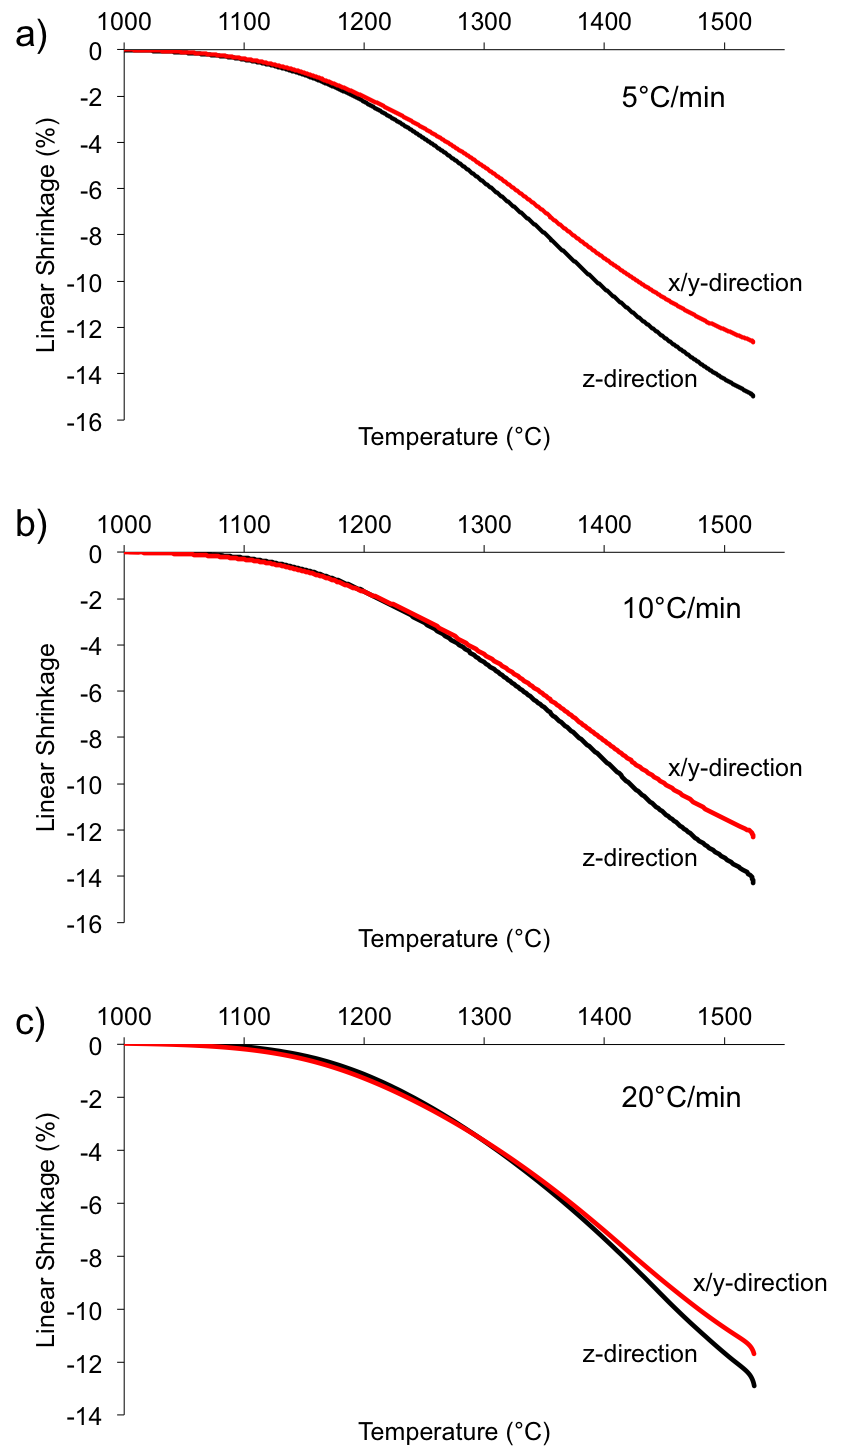
\includegraphics[scale=0.80]{Chapter-6/Figures/Figure1.png}
	\caption{Dilatometry curves of non-aqueous slip cast CT3000LS-SG samples heated at a) 5$^{\circ}$C/min, b) 10$^{\circ}$C/min, and c) 20$^{\circ}$C/min to 1525$^{\circ}$C measured parallel to (z-direction) and perpendicular to (x/y-direction) the capillary force acting during slip casting.}
	\label{Ch6-figure:Figure1}
\end{figure}
%%%

\newpage
%%%
\begin{figure}[H]
	\centering
	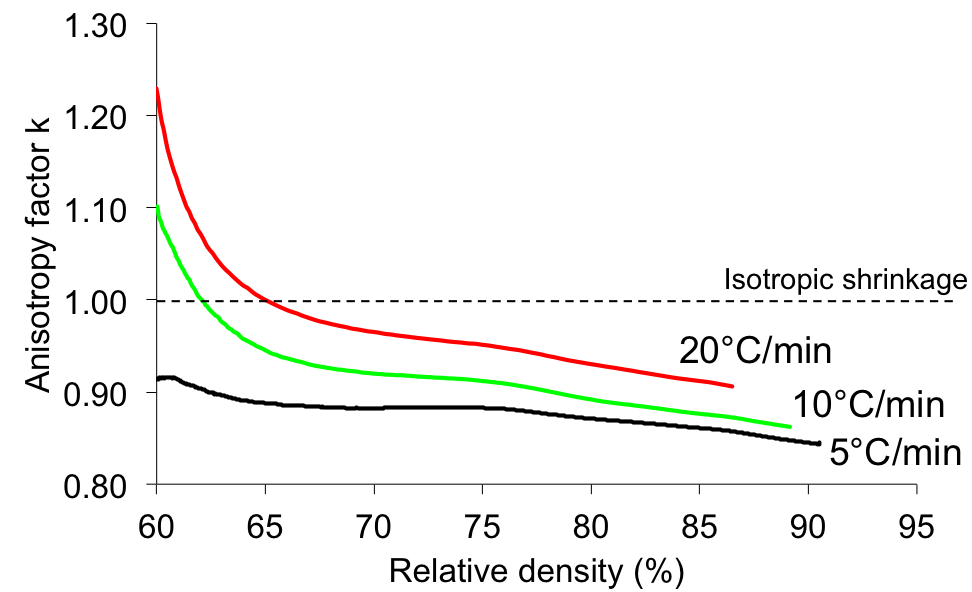
\includegraphics[width=\textwidth]{Chapter-6/Figures/Figure2.png}
	\caption{Development of the shrinkage anisotropy factor for shrinkage, $k$, during densification of non-aqueous slip cast samples as a function of relative density for CT3000LS-SG samples heated at different rates.}
	\label{Ch6-figure:Figure2}
\end{figure}
%%%

\newpage
%%%
\begin{figure}[H]
	\centering
	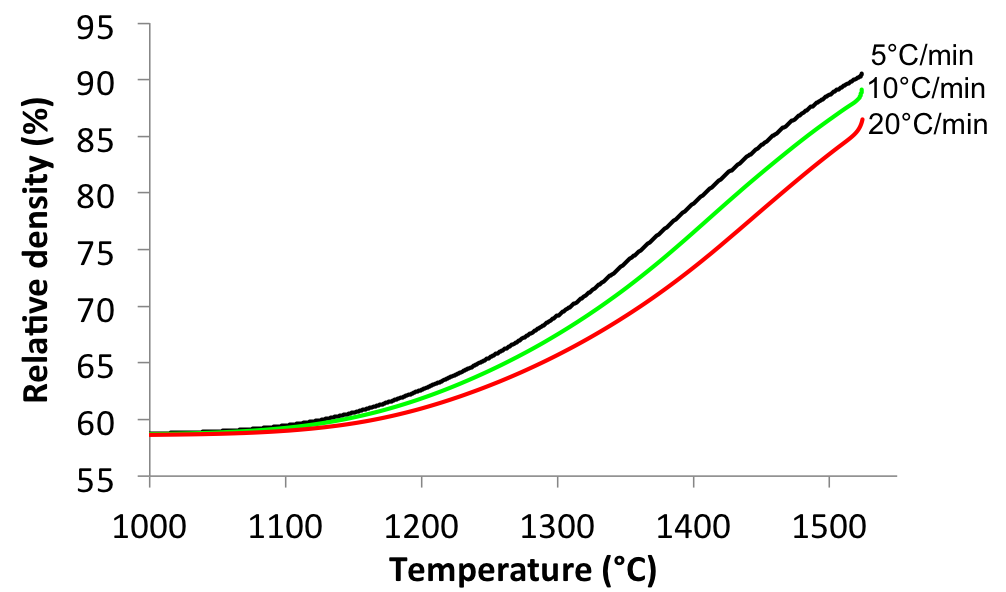
\includegraphics[width=\textwidth]{Chapter-6/Figures/Figure3.png}
	\caption{Development of the relative density corrected for shrinkage anisotropy as a function of temperature for non-aqueous slip cast CT3000LS-SG samples heated at different rates.}
	\label{Ch6-figure:Figure3}
\end{figure}
%%%

\newpage
%%%
\begin{figure}[H]
	\centering
	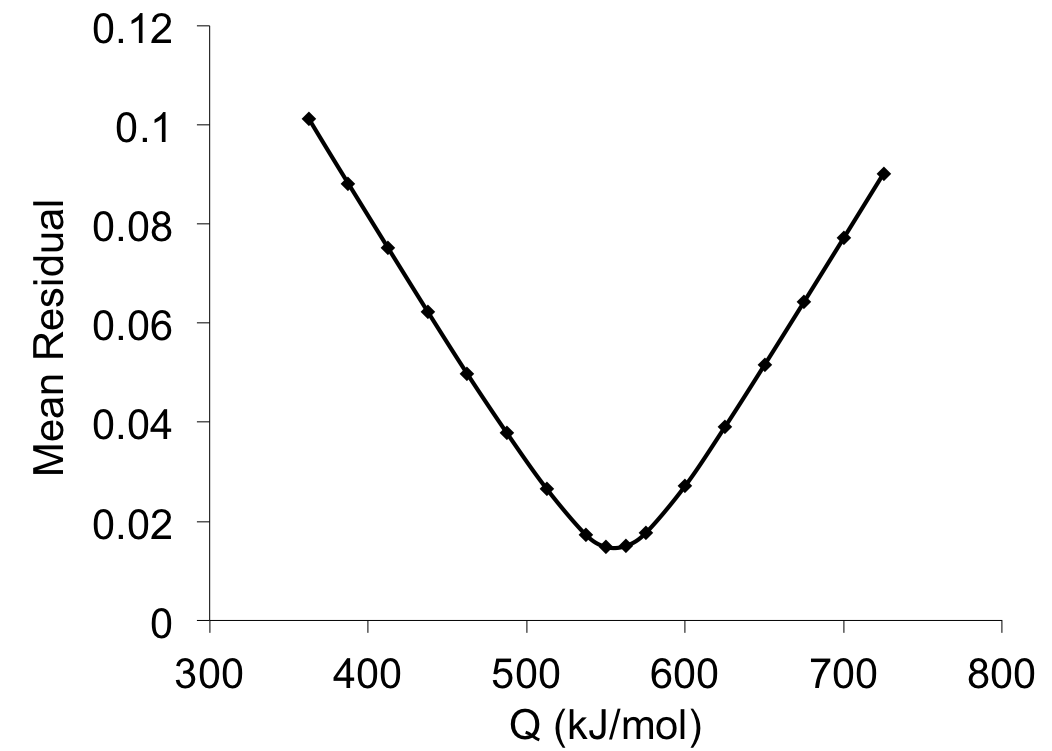
\includegraphics[width=\textwidth]{Chapter-6/Figures/Figure4.png}
	\caption{Mean residuals of the MSC curves assuming different values for $Q$ for non-aqueous slip cast CT3000LS-SG samples.}
	\label{Ch6-figure:Figure4}
\end{figure}
%%%

\newpage
%%%
\begin{figure}[H]
	\centering
	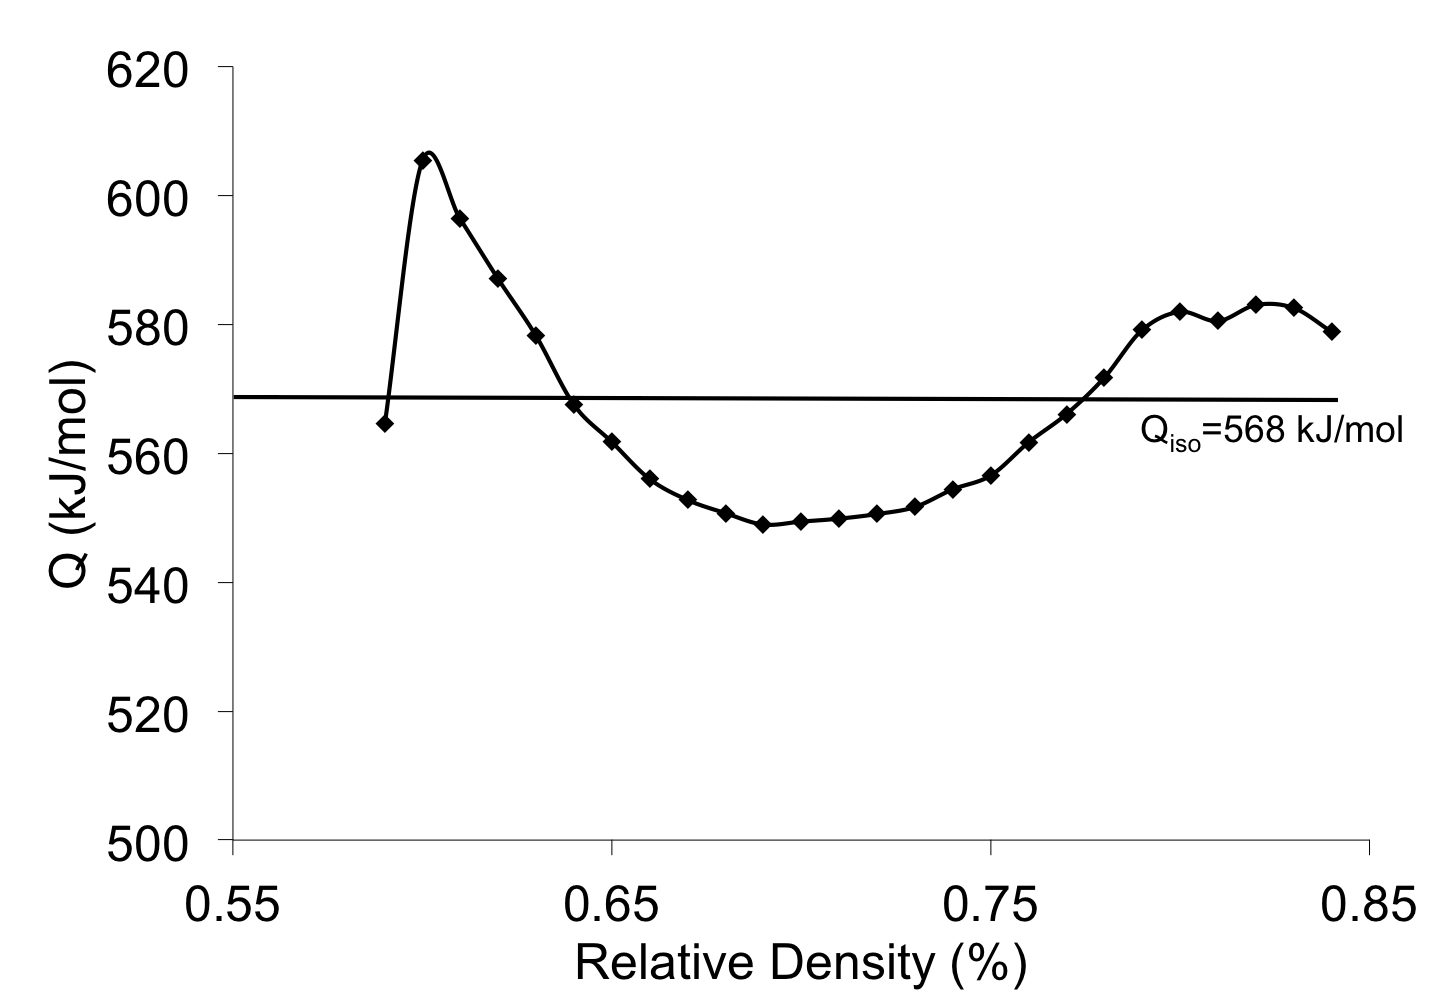
\includegraphics[width=\textwidth]{Chapter-6/Figures/Figure5.png}
	\caption{MSC curves of CT3000LS-SG samples prepared by non-aqueous slip casting using a) the $Q$-value obtained by accounting for shrinkage anisotropy ($Q$=550 kJ/mol) and b) using $Q$-value when shrinkage anisotropy was uncorrected for ($Q$ = 625 kJ/mol).}
	\label{Ch6-figure:Figure5}
\end{figure}
%%%

\newpage
%%%
\begin{figure}[H]
	\centering
	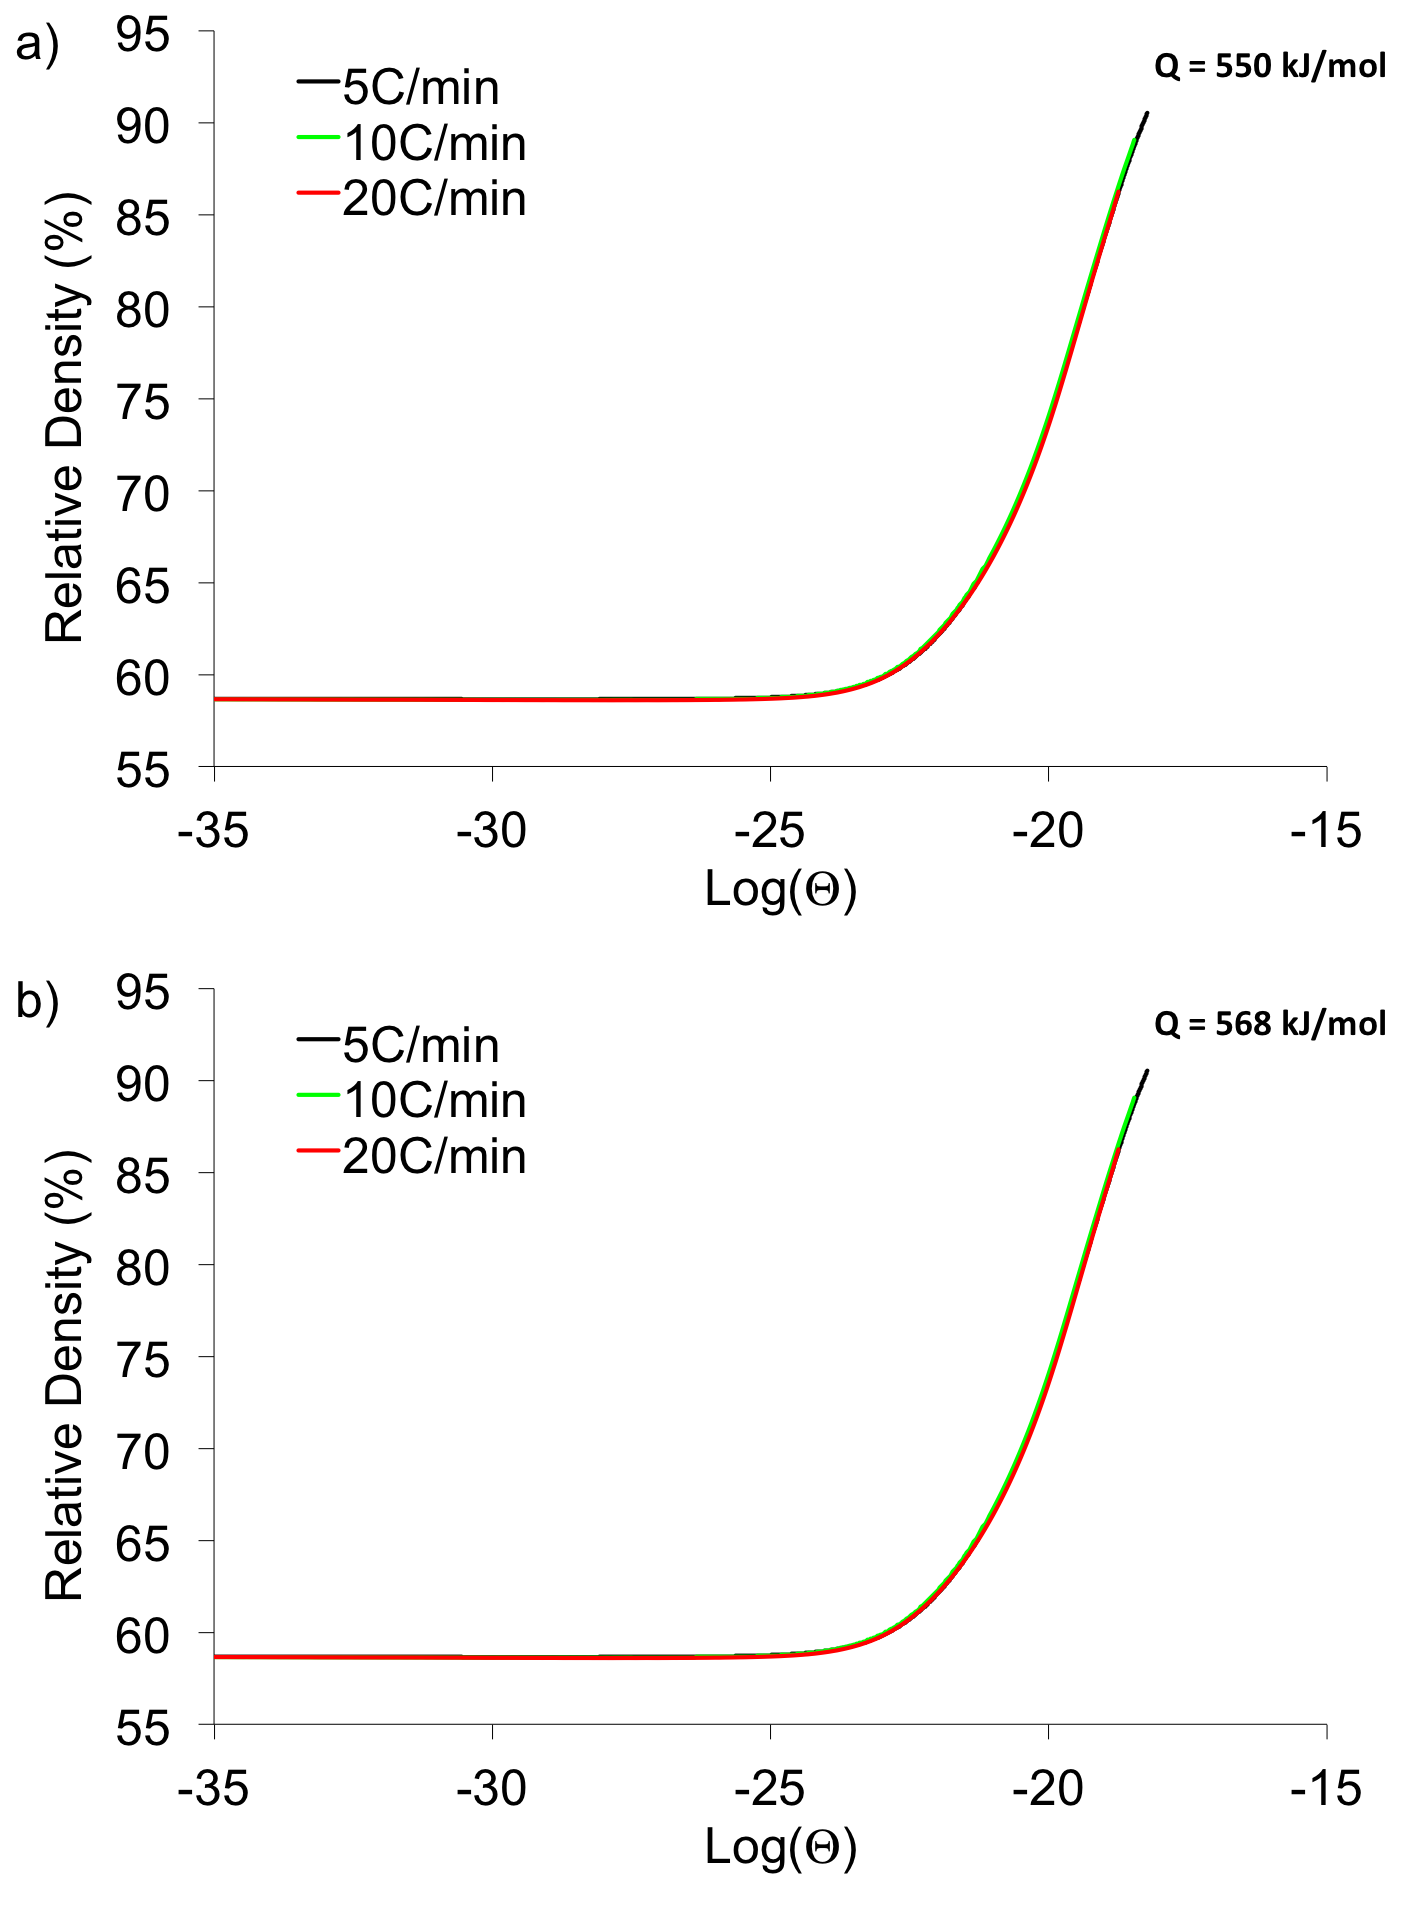
\includegraphics[width=\textwidth]{Chapter-6/Figures/Figure6.png}
	\caption{MSC curves and $Q$-values of CT3000LS-SG samples obtained from the minimum mean residuals for samples prepared by different forming techniques and accounting for shrinkage anisotropy.}
	\label{Ch6-figure:Figure6}
\end{figure}
%%%

\newpage
%%%
\begin{figure}[H]
	\centering
	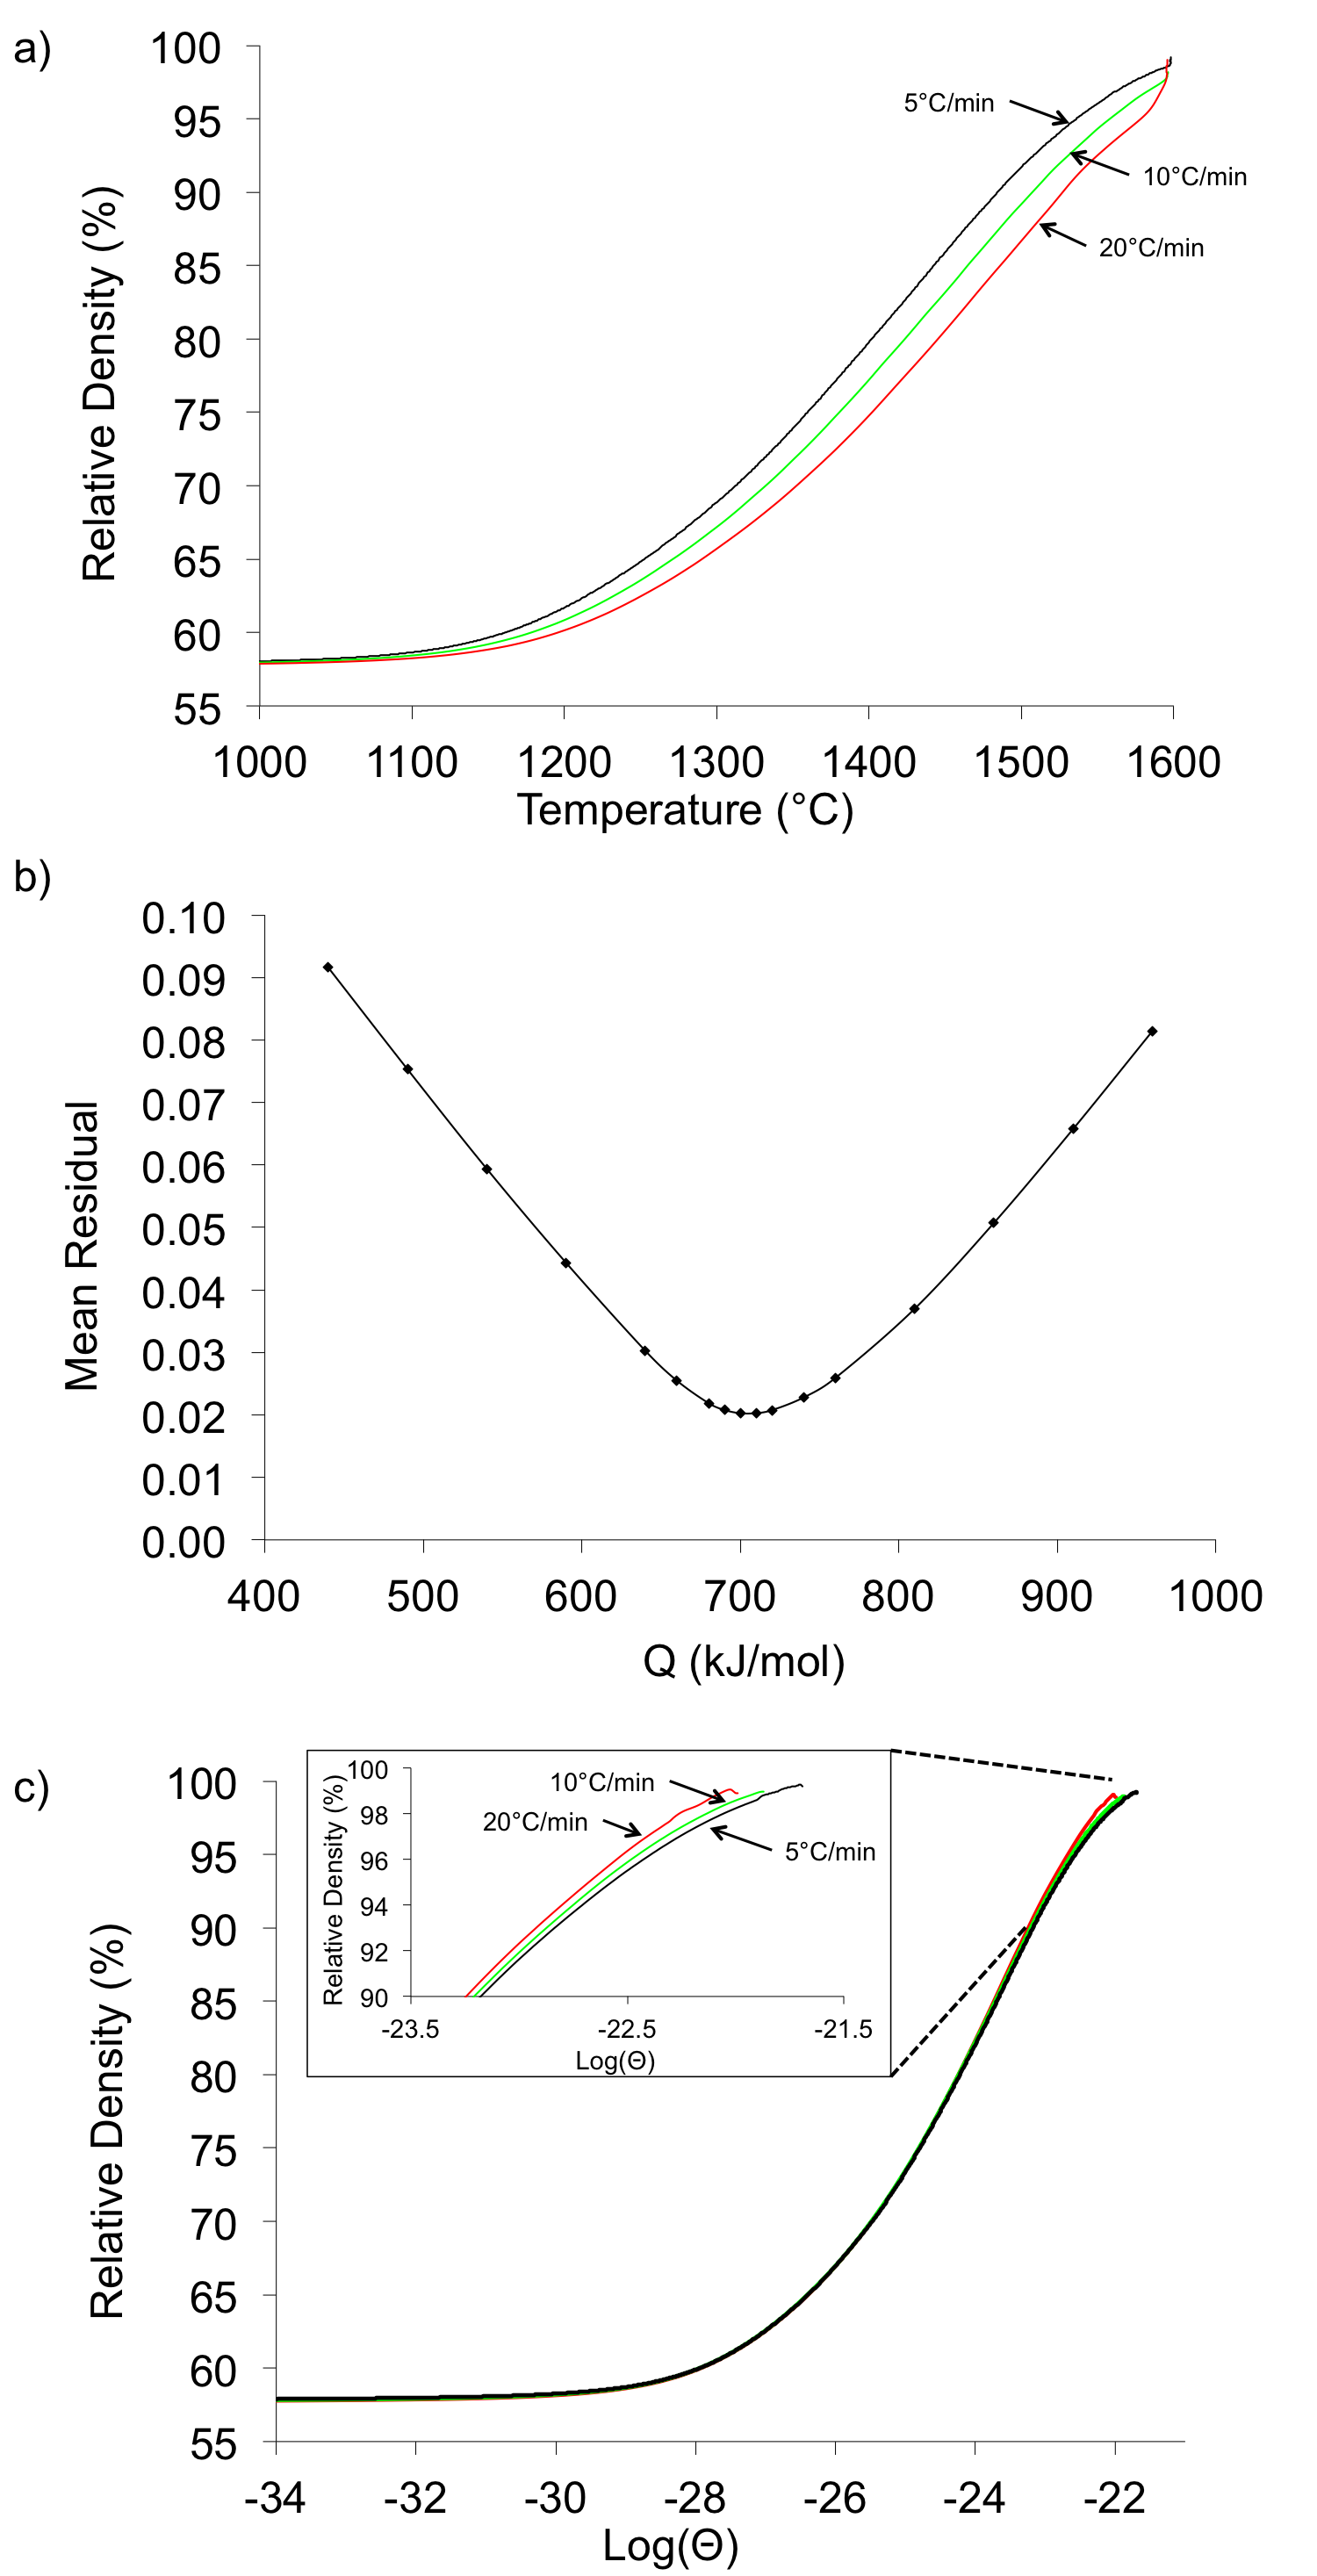
\includegraphics[scale=0.4]{Chapter-6/Figures/Figure7.png}
	\caption{Densification of dry pressed CT3000LS-SG samples at different heating rates, b) mean residuals as a function of $Q$, and c) MSC for $Q$ = 700 kJ/mol obtained from the minimum mean residuals, showing divergence at densities >90\%.}
	\label{Ch6-figure:Figure7}
\end{figure}
%%%

\newpage
%%%
\begin{figure}[H]
	\centering
	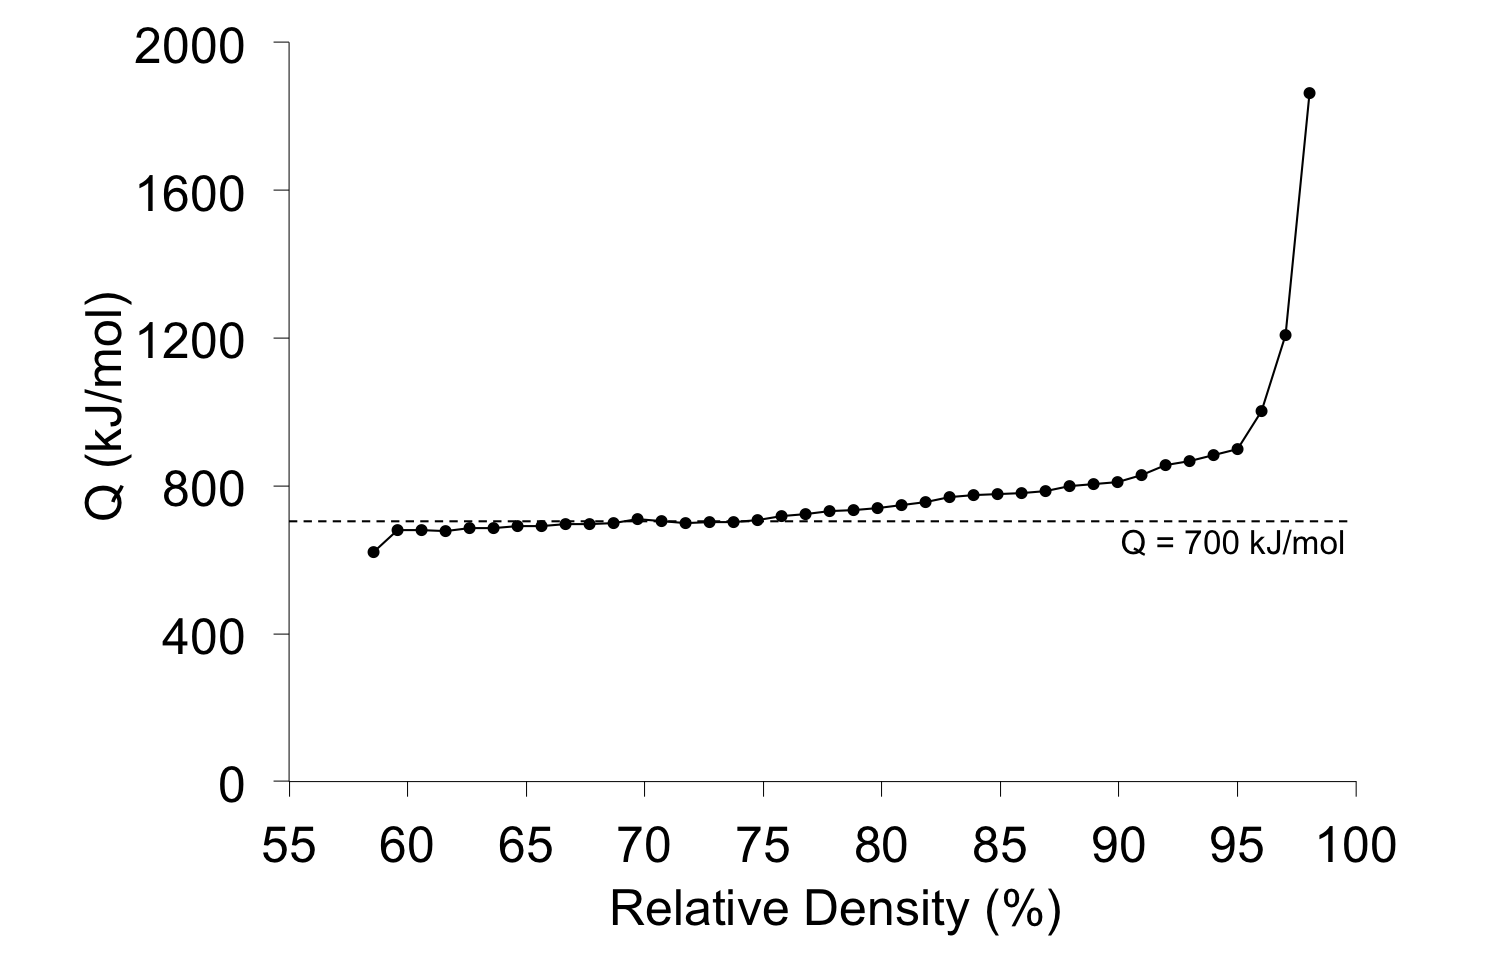
\includegraphics[width=\textwidth]{Chapter-6/Figures/Figure8.png}
	\caption{$Q$-values for dry pressed CT3000LS-SG samples as a function of relative density obtained from iso-density analysis.}
	\label{Ch6-figure:Figure8}
\end{figure}
%%%

\newpage
%%%
\begin{figure}[H]
	\centering
	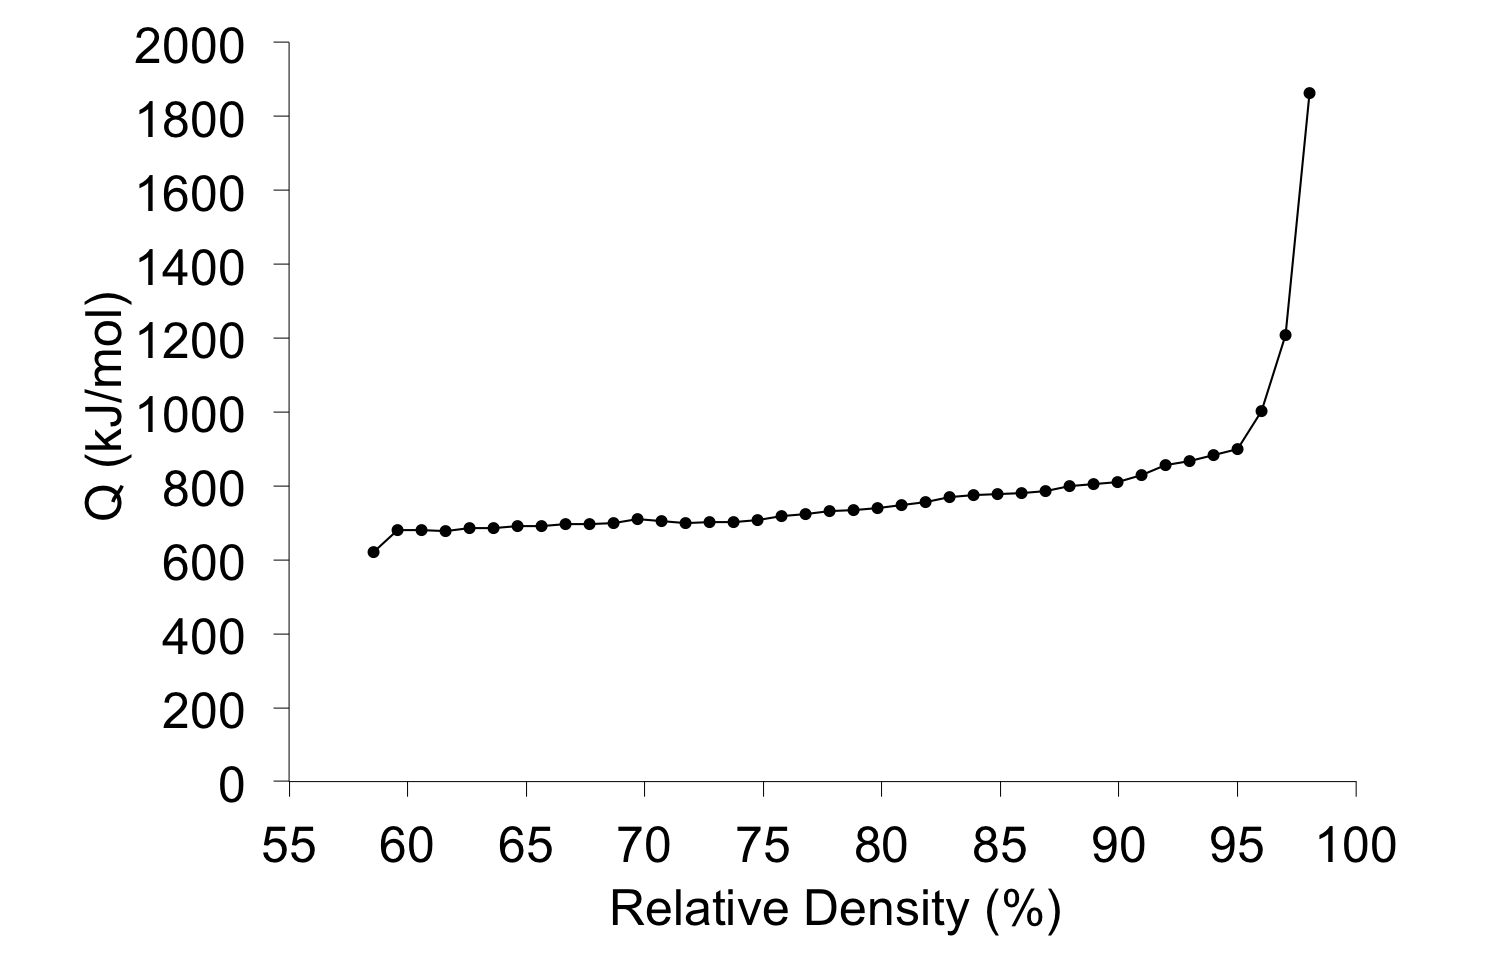
\includegraphics[width=\textwidth]{Chapter-6/Figures/Figure9.png}
	\caption{Development of the microstructural parameters, summarized in the $C$ parameter, as a function of relative density for a dry pressed CT3000LS-SG sample.}
	\label{Ch6-figure:Figure9}
\end{figure}
%%%

\newpage
%%%
\begin{figure}[H]
	\centering
	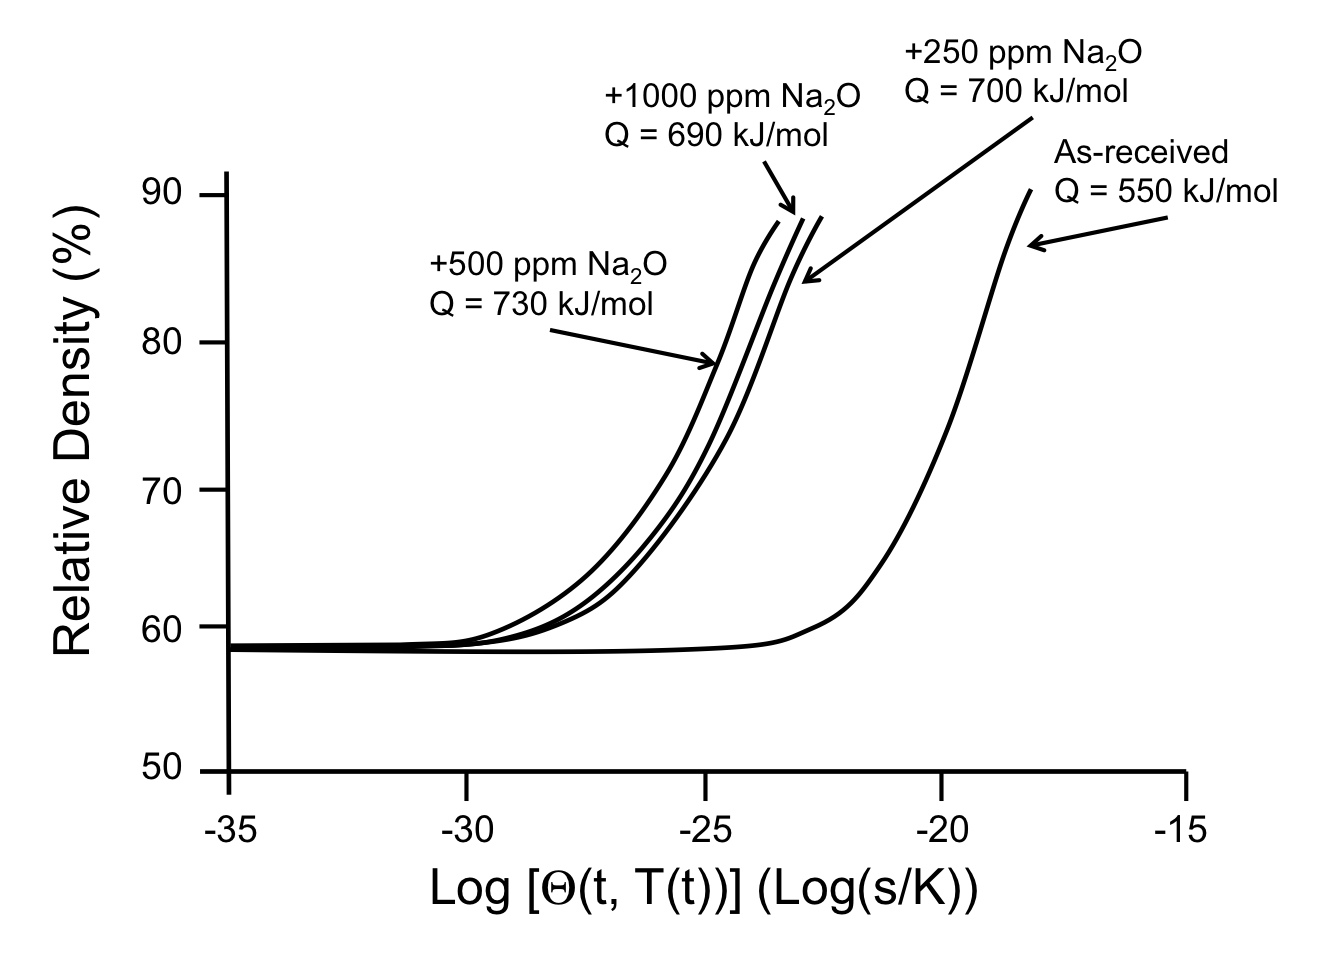
\includegraphics[width=\textwidth]{Chapter-6/Figures/Figure10.png}
	\caption{MSCs and $Q$-values for CT3000LS-SG samples prepared by non-aqueous slip casting with different Na$_{2}$O concentrations.}
	\label{Ch6-figure:Figure10}
\end{figure}
%%%

\newpage
%%%
\begin{figure}[H]
	\centering
	
\includegraphics[width=\textwidth]{Chapter-6/Figures/Figure11.png}
	\caption{Equivalent time/temperature diagram for CT3000LS-SG samples prepared by non-aqueous slip casting heated at 10$^{\circ}$C/min. The contours may be used to predict heat treatments requirements to achieve a desired density.}
	\label{Ch6-figure:Figure11}
\end{figure}
%%%
